\documentclass{article}
\usepackage[margin=1in]{geometry}
\usepackage{tikz}
\usetikzlibrary{shapes.geometric, arrows, positioning}
%For tikz node diagram setup
\pagenumbering{gobble}

\definecolor{mgreen}{HTML}{689562}
\definecolor{mpurp}{HTML}{85678f}
\definecolor{mblue}{HTML}{3C406C}
\definecolor{mgray}{HTML}{6F6F6F}
\tikzset{trapezium stretches=true}
\tikzstyle{source} = [rectangle, rounded corners, minimum width= 2cm, minimum height = 1cm, text = white, text centered, fill = mgray]
\tikzstyle{input} = [trapezium, trapezium left angle=50, trapezium right angle = 130, minimum width = 1.5cm, minimum height=1cm, text centered, text=white, fill=mgreen]
\tikzstyle{routing} = [diamond, minimum width=2cm, minimum height=1cm, aspect = 2, text width = 2cm, text centered, text=white,fill = mblue]
\tikzstyle{processor} = [rectangle, minimum width = 2cm, minimum height = 1cm, text width = 3cm, text = white, fill = mpurp]
\tikzstyle{cable} = [thick, ->, >=latex]
\tikzstyle{usb} = [thick, <->, >=latex]


\begin{document}
\centering
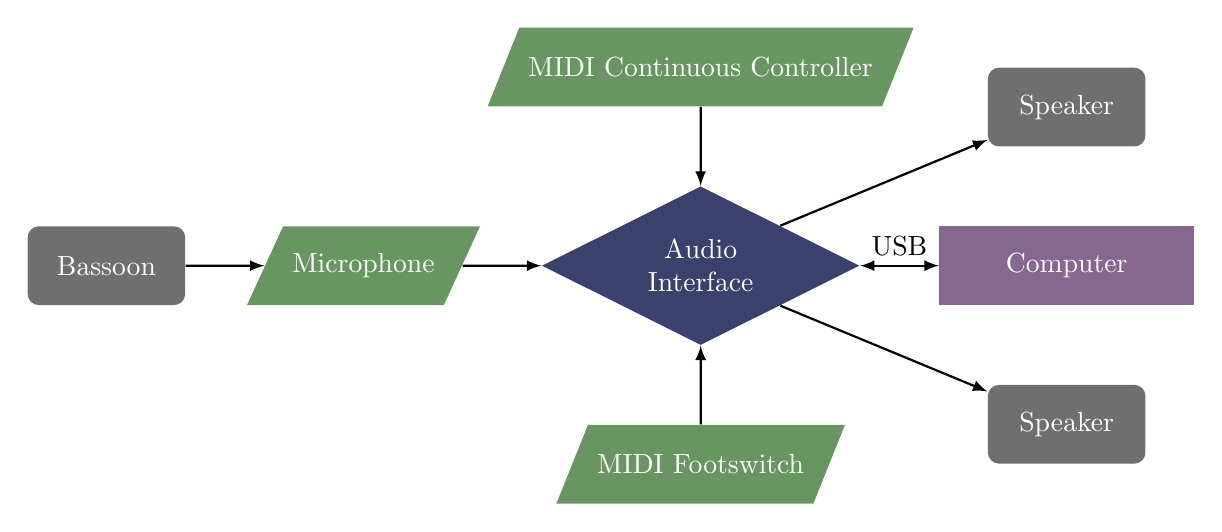
\begin{tikzpicture}[align=center, node distance=1cm]
\node (bsn) [source] {Bassoon};
\node (mic) [input, right = of bsn] {Microphone};
\node (interface) [routing, right = of mic] {Audio Interface};
\node (comp) [processor, text width = 3cm, right = of interface] {Computer};
\node (switch) [input, below = of interface] {MIDI Footswitch};
\node (control) [input, above = of interface] {MIDI Continuous Controller};
\node (speaker1) [source, above = of comp] {Speaker};
\node (speaker2) [source, below = of comp] {Speaker};
\draw [cable] (bsn) -- (mic);
\draw [cable] (mic) -- (interface);
\draw [usb] (interface) -- node[anchor=south]{USB}(comp);
\draw [cable] (switch) -- (interface);
\draw [cable] (control) -- (interface);
\draw [cable] (interface.north east) -- (speaker1);
\draw [cable] (interface.south east) -- (speaker2);
\end{tikzpicture}

\end{document}
